\documentclass[a4paper]{article}

\usepackage[english]{babel}
\usepackage[utf8x]{inputenc}
\usepackage{amsmath}
\usepackage{amsfonts}
\usepackage{graphicx}
\usepackage{subfigure}
\usepackage{url}
\usepackage[colorinlistoftodos]{todonotes}

\title{CS 5785 -- Applied Machine Learning -- Lec.\ 5}
\author{Prof.\ Nathan Kallus, Cornell Tech\\Scribe: TBD}
\date{February, 2017}

\begin{document}
\maketitle

\section{Subset Selection}

Recall from Lecture 2 our discussion of the \emph{bias-variance tradeoff} in class.  Generally, as model complexity increases, there is a change in the variance and bias associated with the model. More complex models, e.g. those with more parameters, smaller \emph{k} in k-Nearest Neighbors, and so on, will have a smaller bias and a greater variance.  These models tend to "overfit" to the data.  On the other hand, less complex models will have a higher bias but a lower variance.  Consider the following examples:
\begin{itemize}
\item Fitting a straight line to your data is a relatively low-complexity model, as there are only two parameters: the intercept and a single coefficient. A straight line will in most cases will have a larger error on the training data than a more complex model.
\item fitting a kth order polynomial to your data is more complex model (assuming k is greater than 1) which has k+1 parameters.  Theoretically, if a large enough value of k is chosen, then the error on the training data can be minimized to 0.
\end{itemize}

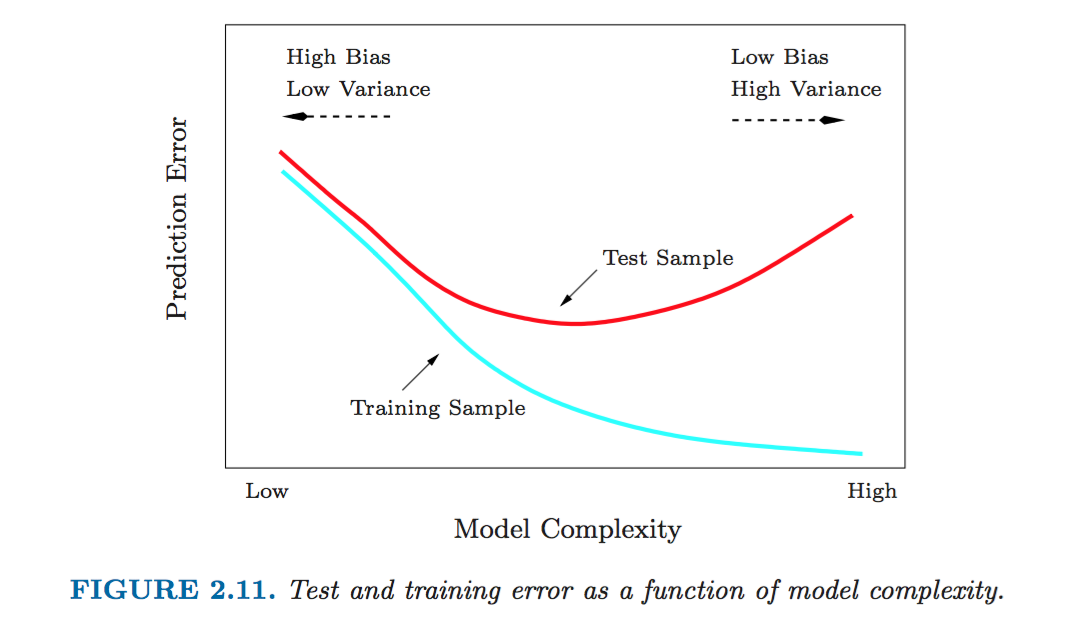
\includegraphics[width=11cm]{bias_var_tradeoff.png}

From these examples, it is clear that model complexity has different effects on the training data and the test data.  Specifically, as model complexity increases, the error on the training data will approach 0.  For the test data there is often some minima for prediction error over different model complexities-- a very low-complexity model may result in high error, as would a high complexity model.  The problem then amounts to finding this optimal complexity at which error on the test data is minimized.  


Subset selection is one approach to help avoid the problem of overfitting with complex models.  The goal is to find a subset of the features that predict the outcome well while avoiding overfitting.  The more features used at training, the more flexibility allowed during training and the greater the risk of overfitting.  Just as perfect accuracy on the training data could be guaranteed in the polynomial example above, it is true that when the number of features is equal to the number of observations that a hyperplane can always be found that fits to all the training points exactly.  Imagine the case with n=2: a straight line can always be found through two points.  To summarize, the idea of subset selection is to leverage structural knowledge to understand which features matter, and to thus learn from fewer data points.

There are two sorts of subset regression covered in this lecture: Best Subset regression and Backward/Forward Stepwise regression.

\emph{Best Subset Regression}: 
Define $support(\beta) = \{j=1,...,p:B_j\neq0\}$ excluding $\beta_0$. Then define the following:

$$\hat{\beta_{bestk}} = \operatorname{arg\,min}_{|supp(\beta)|\leq k} \| Y - X_{\beta} \|^2 - 
\operatorname{arg\,min}_{s \leq \{1,...,\beta\} } \| Y - X_{\beta} \|^2$$
$$\hat{\beta_{bestk}} = \operatorname{arg\,min}_{|supp(\beta)|\leq s} \| Y - X_{\beta} \|^2$$

Recall from ordinary least squares regression that
$$\hat{Y} = \beta^{T}X$$

Then, we see that if $\hat{\beta_{LS}}$ is the least squares estimator for $\beta$, then
$$\hat{\beta_{bestp}} =\hat{\beta_{LS}}$$
 because $|supp(\beta)| \leq p$.
 
 Instead of searching through entire space, we will add/remove features sequentially by assigning a "score" to $\beta_{j}$ for each feature $j$ to decide if its contribution is relatively large or small. In this case, the "score" will be a z-score for each parameter.
 
 For $\hat{\beta_j}$, define the z-score as follows:
 
 
 As a rule of thumb, we consider significant features to be those with a z-score of magnitude 2 (either positive or negative). We can use these scores along with an algorithm for feature selection to control model complexity with forward and backward stepwise regression.
 
 \emph{Backward Stepwise Regression}:
 
 \emph{Forward Stepwise Regression}:
 
 How do we decide when to terminate either of these algorithms?  There are several different techniques one can apply.  For instance, we might want to stop when all features are significant, i.e. when the absolute value of all z-scores is at least 2.  We could apply any of a number of model fit tests at each iteration and stop when we are satisfied with the model fit.  Perhaps the best approach is to use cross-validation to decide the appropriate number of iterations for each of these algorithms.  
 
 \emph{Side notes on Cross-Validation}:
 
 
 

\section{Shrinkage}
\todo{Write Me!}




% Examples from last year's notes

\clearpage
\todo{Delete the other sections}
\section{Newton-Raphson}
Logistic regression models are usually fit by maximum likelihood. As described at the end of last lecture, to maximize the log likelihood $\ell(\beta)$ we will make use of both its first and second order derivatives.  Let's first review what we can do with just first order derivatives and then see what the second order derivatives have to offer.
The sequence of panels in Fig.\ \ref{fig:newton} from Wikipedia illustrates Newton's method for finding a root (zero crossing) of a function (shown in blue). 

\begin{equation}
\ell(\beta) = \sum_{i=1}^N \left \{ y_i \beta ^\top x_i -  log(1+ e^{\beta ^\top x_i}) \right \}
\label{eqn:llgrad}
	\end{equation}
    
\begin{figure}
\centering
\subfigure[Start with a guess $x_1$, find the tangent line using the first derivative, extrapolate to get next guess $x_2$.]{
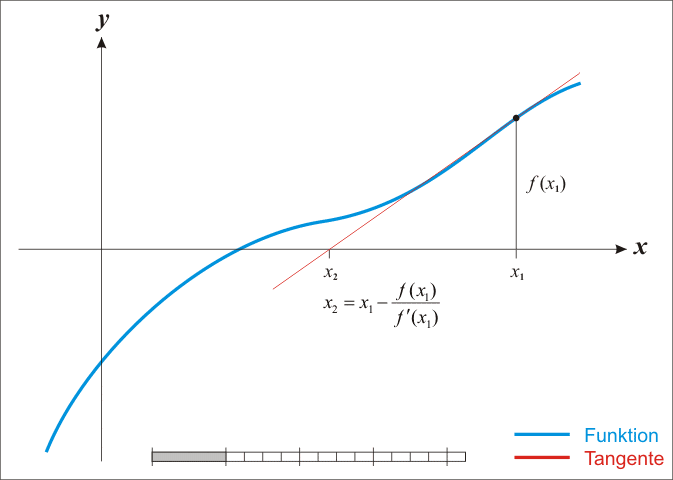
\includegraphics[width=0.45\textwidth]{NewtonIteration_Ani1.png}}
\quad
\subfigure[Repeat this process to get $x_3$, which as we can see overshoots in this case.]{
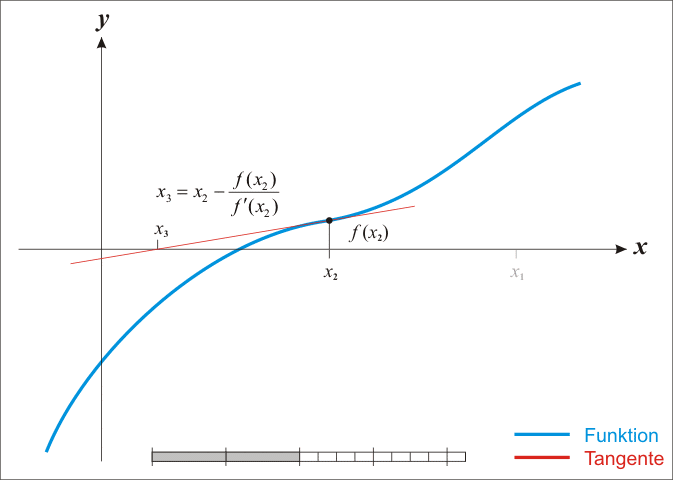
\includegraphics[width=0.45\textwidth]{NewtonIteration_Ani2.png}}

\subfigure[Keep iterating]{
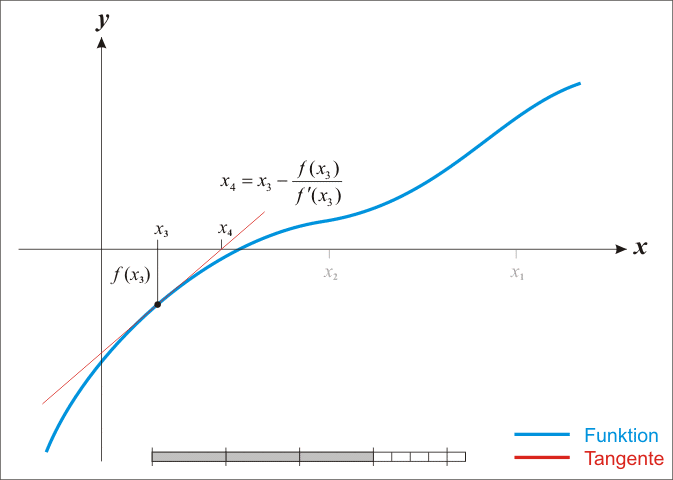
\includegraphics[width=0.45\textwidth]{NewtonIteration_Ani3.png}}
\quad
\subfigure[until a sufficiently accurate value is reached.]{
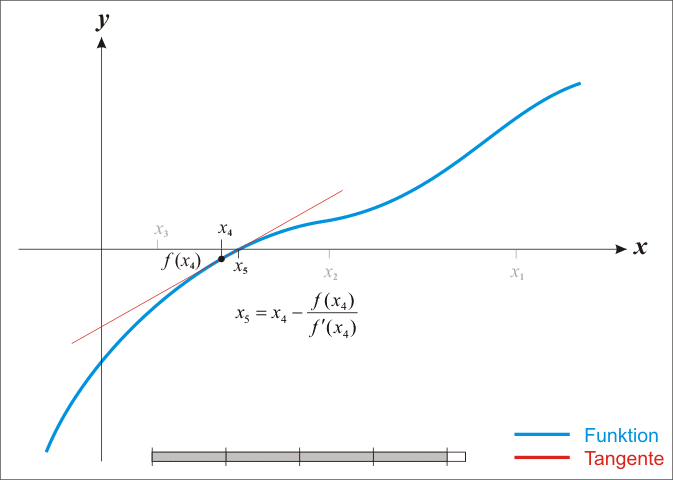
\includegraphics[width=0.45\textwidth]{NewtonIteration_Ani4.png}}
\caption{Illustration of Newton's method for finding a root. (Wikipedia)}
\label{fig:newton}
\end{figure}

In our case we wish to solve the related problem of finding the maximum of a function.  We will do this using both the first and second derivatives as shown in Fig.\ \ref{fig:newton2} for a 1D function.  Instead of fitting a tangent line to the function to generate the next guess, we fit a local quadratic approximation, i.e., a function that has the same 1st and 2nd derivatives as the function in the neighborhood of a guess.  In higher dimensions, as with our log likelihood $\ell(\beta)$ where $\beta\in\mathbb{R}^{p+1}$, the counterparts to the 1st and 2nd derivatives are the gradient and the Hessian, respectively.,

\begin{figure}
\centering
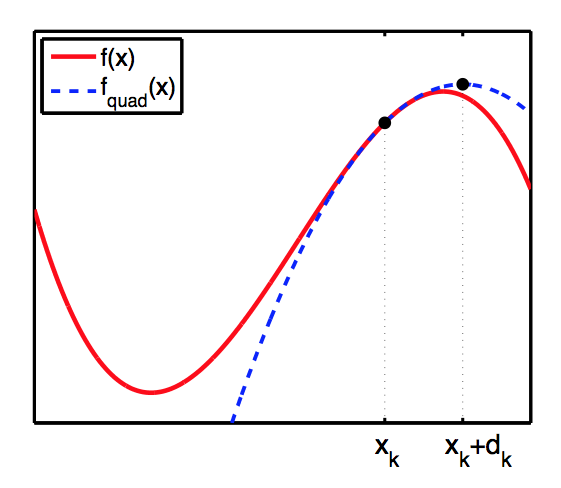
\includegraphics[width=0.5\textwidth]{newton_noncvx.png}
\caption{Finding a local maximum of a function $f(x)$ using a quadratic approximation.  We start with a guess at $x_k$.  Using both the 1st and 2nd order derivatives we fit a quadratic approximation to the function at that point.  That function $f_{\text{quad}}(x)$, is equivalent to the 2nd order Taylor series approximation of $f(x)$ around $x_k$.  We can easily solve for the maximum of this function and obtain the next guess for the maximum, $x_k+d_k$. We repeat this process until convergence. (Murphy)}
\label{fig:newton2}
\end{figure}

As we saw in the last lecture, the gradient of the log likelihood is given by
\begin{equation}
\frac{\partial \ell(\beta)}{\partial \beta} = \sum_{i=1}^N x_i (y_i - p(x_i;\beta))
\label{eqn:llgrad}
	\end{equation}
Note that the gradient is a length $p+1$ vector.  We can see from this expression that the gradient can be expressed as a sum of feature vectors $x_i\in\mathbb{R}^{p+1}$, $i=1,\ldots,N$, weighted by $y_i-p(x_i;\beta)$.  We can interpret that weight as a signed error, since $p(x_i;\beta)$, the posterior probability, aims to approximate $y_i$.

It is straightforward to show that the Hessian of $\ell(\beta)$, which is a $(p+1)\times(p+1)$ matrix, is given by
$$
\frac{\partial^2 \ell(\beta)}{\partial \beta\partial \beta^\top} = -\sum_{i=1}^N x_i x_i^\top p(x_i;\beta)\left(1-p(x_i;\beta)\right)
$$
This matrix is a sum of terms of the form $x_i x_i^\top$ weighted by $p(x_i;\beta)(1-p(x_i;\beta))$ and it characterizes the curvature of the function we're trying to minimize. Each $x_i x_i^\top$ term is the \textit{outer product} of $x_i$ with itself, resulting in a symmetric matrix of size $(p+1)\times(p+1)$.  We will see soon that this is closely related to how we compute the \emph{covariance matrix} for $\left\{x_i\right\}_1^N$. The scalar weight $p(x_i;\beta)(1-p(x_i;\beta))$ has a small value when $p(x_i;\beta)$ is close to $y_i$. If $p(x_i;\beta)$ is close to $1$ then $1 - p(x_i;\beta)$ is close to $0$ and vice versa, which means that if the approximation is good at least one multiplier in the expression $p(x_i;\beta)(1-p(x_i;\beta))$ is close to $0$. As a result, the entire expression has a very low value far from the decision boundary. If $p(x_i;\beta)$ is a bad approximation of $y_i$ there is a higher chance that the classification is incorrect and as such $p(x_i;\beta)$ is closer to $0.5$, $1 - p(x_i;\beta)$ is also close to $0.5$ making the entire expression close to $0.25$. If we look back at the Hessian we can now see that the sum emphasizes $x_i$s that we are less certain of their classification making the contribution to the Hessian  larger when the choice of $\beta$ results in a poor decision boundary. 


\subsection{Iterative Reweighted Least Squares (IRLS)}
In IRLS we start by picking a random choice for $\beta$ and apply a "Newton update" to get a better $\beta$. We continue taking Newton steps until we reach convergence. 
A Newton update is:
$$\beta^{new} = \beta^{old} - \left(\frac{\partial^2 \ell(\beta)}{\partial \beta\partial \beta^\top}\right)^{-1}\frac{\partial \ell(\beta)}{\partial \beta}$$
in which the derivatives are evaluated at $\beta=\beta^{old}$.  If we put this in matrix notation we get:
$$\frac{\partial \ell(\beta)}{\partial \beta} = \mathbf{X}^\top(\mathbf{y}-\mathbf{p})$$
$$\frac{\partial^2 \ell(\beta)}{\partial \beta\partial \beta^\top} = -\mathbf{X}^\top \mathbf{W}\mathbf{X}$$
Where:
\begin{itemize}
  \item $\mathbf{y}$ is a vector of all the $y_i$s.
  \item $\mathbf{X}\in\mathbb{R}^{N\times (p+1)}$ is the matrix of all the feature vectors $x_i$s.
  \item $\mathbf{p}$ is a vector of the $p(x_i;\beta)s$.
  \item $\mathbf{W}\in\mathbb{R}^{N\times N}$ is a diagonal weighting matrix containing the values of $p(x_i;\beta)(1-p(x_i;\beta))$ on the diagonal.
\end{itemize}
When we write the Newton update using this notation we get:
$$\beta^{new} = \beta+(\mathbf{X}^\top \mathbf{W}\mathbf{X})^{-1}\mathbf{X}^\top(\mathbf{y}-\mathbf{p})$$
$$\Downarrow$$
\begin{center}{(Multiply $\beta$ by $(\mathbf{X}^\top \mathbf{W}\mathbf{X})^{-1}(\mathbf{X}^\top \mathbf{W}\mathbf{X})$ which is the same as not changing it)}\end{center}
$$\beta^{new} = (\mathbf{X}^\top \mathbf{W}\mathbf{X})^{-1}(\mathbf{X}^\top \mathbf{W}\mathbf{X})\beta+(\mathbf{X}^\top \mathbf{W}\mathbf{X})^{-1}\mathbf{X}^\top(\mathbf{y}-\mathbf{p})$$
$$\Downarrow$$
\begin{center}(Factor out $(\mathbf{X}^\top \mathbf{W}\mathbf{X})^{-1}\mathbf{X}^\top \mathbf{W}$)\end{center}
$$\beta^{new} = (\mathbf{X}^\top \mathbf{W}\mathbf{X})^{-1}\mathbf{X}^\top \mathbf{W}(\mathbf{X}\beta+\mathbf{W}^{-1}(\mathbf{y}-\mathbf{p}))$$
$$\Downarrow$$
$$\beta^{new} = (\mathbf{X}^\top \mathbf{W}\mathbf{X})^{-1}\mathbf{X}^\top \mathbf{W}\mathbf{z}$$
in which $\mathbf{z}=\mathbf{X}\beta+\mathbf{W}^{-1}(\mathbf{y}-\mathbf{p})$. We call $\mathbf{z}$ the \textit{adjusted response}.\\
In every IRLS iteration we solve this equation with a new set of $\mathbf{p}$, $\mathbf{W}$ and $\mathbf{z}$. We get:
$$\beta^{new}\leftarrow\underset{\beta}{\arg\min}(\mathbf{z}-\mathbf{X}\beta)^\top \mathbf{W}(\mathbf{z}-\mathbf{X}\beta)$$
We iterate this step until  convergence. 
This is named \emph{Iteratively Reweighted Least Squares} since in every iteration it solves a weighted least squares problem.

One remaining question is, how do we initialize $\beta$? Starting with $\beta=0$ is often OK.  Another option is to use multiple randomized restarts to reduce the chances of getting stuck at a local maximum.

\begin{itemize}
\item Pros: Its fast
\end{itemize}



\begin{itemize}
\item Cons: For each iteration need to invert a large matrix.
\item Cons: Need to include all observations in this matrix.
\end{itemize}

\begin{figure}
\centering
\subfigure{
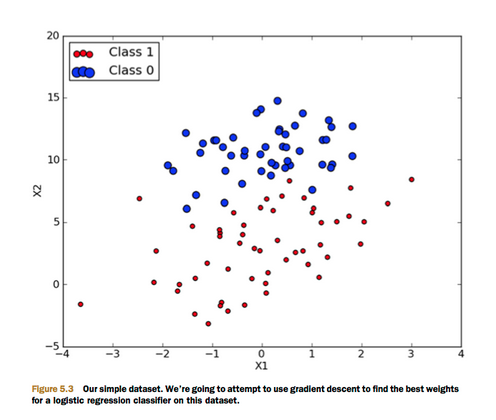
\includegraphics[width=0.45\textwidth]{HarringtonExample1.png}}
\quad
\subfigure{
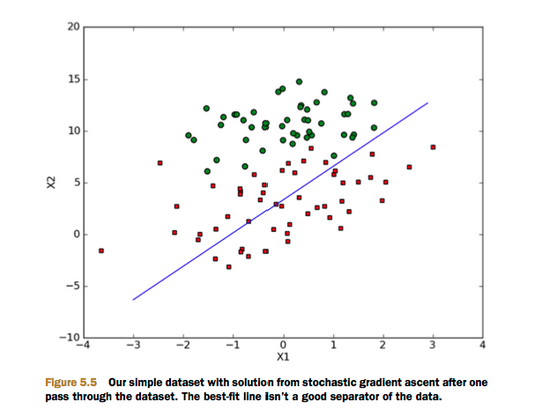
\includegraphics[width=0.45\textwidth]{HarringtonExample2.png}}

\subfigure{
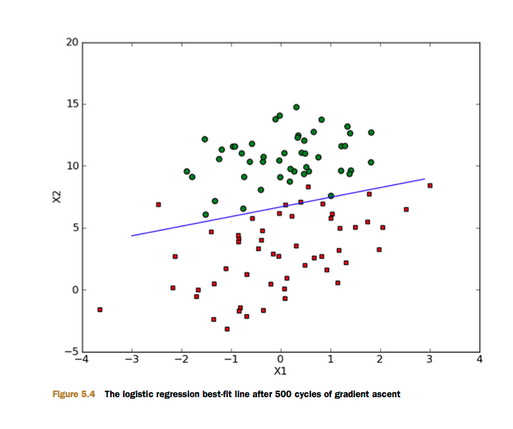
\includegraphics[width=0.45\textwidth]{HarringtonExample3.png}}
\quad
\caption{Logistic regression example (Harrington)}
\label{fig:Harrington}
\end{figure}


\section{Online Learning}
\subsection{Stochastic Gradient Descent}
IRLS is called a ``batch'' method since it has all the necessary data in advance, but that is not always possible or available.  For example, the data could be too big to fit into memory. Online learning updates $\beta$ every step based on individual streamed instances, as opposed to IRLS that uses all the data in every step.  \emph{Stochastic Gradient Descent} (SGD) is an example of an online learning or streaming method that uses the following update step with \emph{step size} or \emph{learning rate} $\alpha$:
$$\beta^{new}\leftarrow \beta^{old}-\alpha x_i (y_i - p(x_i;\beta))$$
Compared to the exact expression for the gradient in Eqn.\ (\ref{eqn:llgrad}), SGD updates $\beta$ per data point rather than summing the gradient contributions over the entire data set.  If the data point was classified correctly the boundary doesn't change, if not we use the update rule above to update it. \todo[inline, color=green!40]{Technically that's perceptron learning; in this expression the update is proportional (including sign)  to the discrepancy between the ground truth and the estimated posterior probability.} How do we choose the step size $\alpha$?  This is left as an exercise for the reader.

This algorithm is closely related to Rosenblatt's \emph{Perceptron Learning Algorithm} (HTF \S4.5.1), which is hard thresholded and doesn't maintain probability estimates.  See an example here: \url{http://www.youtube.com/watch?v=vGwemZhPlsA} (``Perceptron Learning Rule'').  The LMS algorithm of Widrow and Hoff is also an example of SGD. SGD are also used in training neural networks.

\textbf{Perceptron Algorithm }


\begin{figure}
\centering
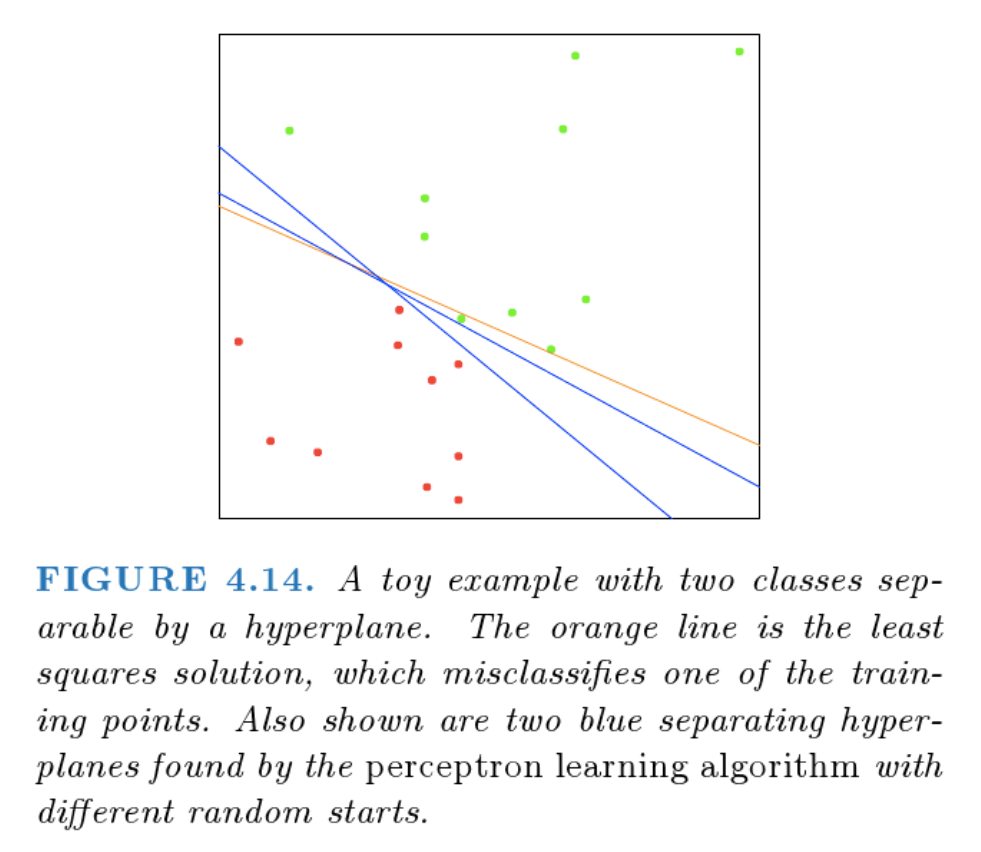
\includegraphics[width=0.75\textwidth]{sep_hyperplane}
\label{fig:sep_hyperplane}
\end{figure}

\subsection{Thoughts on Separating Hyperplanes}
As shown in HTF Fig.\ 4.14, given two classes that are linearly separable, there exists an infinite family of separating lines/planes/hyperplanes between the classes.  The figure shows solutions found via perceptron learning with different initializations.  Which solution is best?  Our intuition suggests we should choose the line with the furthest  perpendicular distance from the closest data points from each class, since this might prevent overfitting. How do we translate that into an algorithm?  We will tackle this question later in the semester when we discuss \emph{support vector machines}.

\subsection{Kernels: a Preview}
Note that so far we have just been using the input variables $X$ in their raw form (apart from adding the 1 to the front). A whole new frontier of algorithms awaits us if we supplement $x$ by squares and cross products of its variables like $x_1^2,x_2^2, x_1x_2$, etc. This hints at the idea of a \textit{kernel}, a mapping through which we can augment the representation by adding dimensionality. This is particularly useful when dealing with points that are not linearly separable, as in the XOR problem. We will discuss kernels later in the semester.






\end{document}
